\documentclass[11pt]{article}
\usepackage{geometry}
\geometry{a4paper, top=20mm, left=10mm, right=10mm, bottom=20mm}
\usepackage{graphicx}
\usepackage{amsmath,amssymb,amsthm}
\usepackage{amssymb}
\usepackage[utf8]{inputenc}
\usepackage{fancyhdr}
\usepackage{lastpage}
\usepackage{enumerate}
\usepackage{enumitem}
\usepackage{tikz}
\usetikzlibrary{shapes.geometric}
\usepackage{multicol}
\usepackage{subcaption}
\usepackage{ifthen}
%------------------------------------------ preamble
%----- fancyhdr
\fancyhead[R]{Übungsgruppe: 2 (Do 12-14)}
\fancyhead[C]{Name: Maurice Wenig}
\fancyhead[L]{Matrikelnummer: 178049}
\fancyfoot{}
\rfoot{Seite \thepage\ von \pageref{LastPage}}
\pagestyle{fancy}
%----- aufgaben
\newtheoremstyle{break}{}{5mm}{}{}{\bfseries}{}{0mm}
{\textbf{\thmname{#1}\thmnumber{ #2:} \thmnote{\textit{#3}}\newline}}
\theoremstyle{break}
\newtheorem{task}{Aufgabe}
%----- new commands
\newcommand{\Romannumeral}[1]{\MakeUppercase{\romannumeral #1}}
%----- tikz automata
\usetikzlibrary{arrows, automata, positioning}
%------------------------------------------ main
\begin{document}
%----- title
\begin{center}
\Large{Automaten und Berechenbarkeit}\\
\large{3. Übungsserie}
\end{center}
%----- tasks
\begin{task}
\hfill\vspace{-5mm}
\begin{enumerate}[align=left]
\item[Symmetrie:] \hfill\vspace{-4mm}\begin{flalign*}
u\sim_L v &\iff \forall w\in\Sigma^*\ (uw\in L\iff vw\in L)&\\
&\iff \forall w\in\Sigma^*\ (vw\in L\iff uw\in L)&\\
&\iff \underline{v\sim_L u} &
\end{flalign*}
\item[Transitivität:] \hfill\vspace{-4mm}\begin{flalign*}
x\sim_L y \land y\sim_L z &\iff \forall w\in\Sigma^*\ (xw\in L\iff yw\in L) \land \forall w\in\Sigma^*\ (yw\in L\iff zw\in L) &\\
&\iff \forall w\in\Sigma^*\ ((xw\in L\iff yw\in L)\land (yw\in L\iff zw\in L)) &\\
&\iff \forall w\in\Sigma^*\ (xw\in L\iff yw\in L\iff zw\in L) &\\
&\implies \forall w\in\Sigma^*\ (xw\in L\iff zw\in L)\iff \underline{x\sim_L z}
\end{flalign*}
\item[Reflexivität:] \hfill\vspace{-4mm}\begin{flalign*}
u\sim_L u &\iff \forall w\in\Sigma^*\ (\underbrace{uw\in L\iff uw\in L}_{Taut.})&
\end{flalign*}
\end{enumerate}
\end{task}

\begin{task}
\hfill\vspace{-5mm}
\begin{enumerate}[label={(\alph*)}]
\item $\{[\lambda], [a], [aa], [aaa], [aaaa]\}$
\item $\{[\lambda], [a], [ab], [aba]\}$
\item $\{[\lambda], [b], [bb], [bba], [bbaa]\}$
\end{enumerate}
\end{task}

\begin{task}
\hfill\vspace{-2mm}\\
\begin{tabular}{rl}
IA:&$\left\vert w\right\vert=1$, $\delta^*((q,p),w) = \delta((q,p),w) \stackrel{\mbox{\tiny def.}}{=} (\delta(q,w), \delta(p,w)) = (\delta^*(q,w), \delta^*(p,w))$\\
IV:&für $w$ gilt: $\delta^*((q,p),w) = (\delta^*(q,w), \delta^*(p,w))$\\
IB:&für $w\cdot a,\ a\in\Sigma$ gilt: $\delta^*((q,p),w\cdot a) = (\delta^*(q,w\cdot a), \delta^*(p,w\cdot a))$\\
IS:&$w\rightarrow w\cdot a$\\
&$\delta^*((q,p),w\cdot a)=\delta(\delta^*((q,p),w), a)\stackrel{\mbox{\tiny IV}}{=} \delta((\delta^*(q,w), \delta^*(p,w)), a) = (\delta((\delta^*(q,w), a), \delta(\delta^*(p,w), a))$\\
&$=\underline{\underline{(\delta^*(q,w\cdot a), \delta^*(p,w\cdot a))}}$
\end{tabular}\vspace{3mm}
\end{task}

\begin{task}
\hfill\vspace{-5mm}
\begin{enumerate}[label={(\alph*)}]
\item \hfill\vspace{-5mm}\\
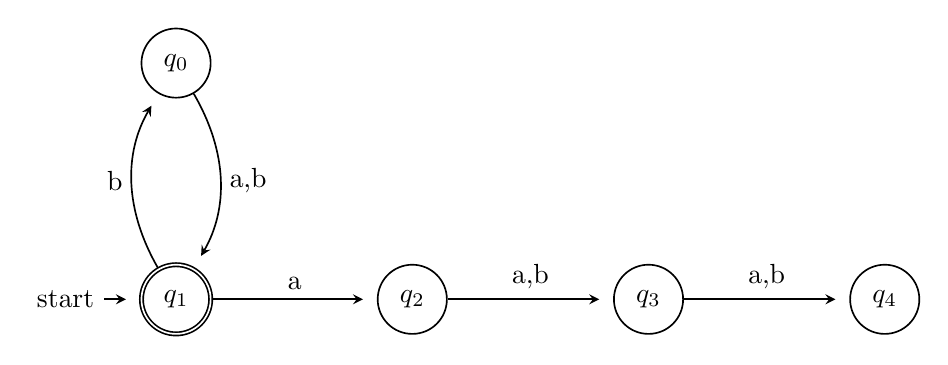
\begin{tikzpicture}[->, > = stealth, shorten > = 5 pt, node distance = 3cm, semithick]

\node[state, initial, accepting]		(1)						{$q_1$};
\node[state]							(0) [above of=1]			{$q_0$};
\node[state]							(2) [right of=1] 		{$q_2$};
\node[state]							(3) [right of=2] 		{$q_3$};
\node[state]							(4) [right of=3] 		{$q_4$};

\path	(0)	edge[right, bend left]		node {a,b}		(1);
\path	(1)	edge[left, bend left]		node {b}			(0);
\path	(1)	edge[above]					node {a}			(2);
\path	(2)	edge[above]					node {a,b}		(3);
\path	(3)	edge[above]					node {a,b}		(4);

\end{tikzpicture}
\end{enumerate}
\end{task}
\end{document}
